\begin{pastexam}[label={px:gk3-111-ds-03}]{高考三級資訊處理 111 年 第三題}
（申論；25 分）

一個二元搜尋樹（Binary search tree）的前序追蹤（Preorder traversal）結果如下：14, 4, 3, 9, 7, 5, 15,
18, 16, 17, 20\\
請建構此二元搜尋樹。接著利用如下 C 語言對二元樹節點的宣告，使用 C 語言寫一遞迴程式
sortTree（NODEPTR tree），輸入二元樹的根節點，來處理此二元樹的節點資料，並將資料依由小至大輸出。
（25 分）
\begin{minted}[fontsize=\small, frame=single]{c}
struct node{
    int info;
    struct node *left;
    struct node *right;
}
typedef struct node *NODEPTR;

void sortTree(NODEPTR tree){

}
\end{minted}
\end{pastexam}

\begin{pastsoln}
原卷的 \texttt{struct node\{...\}} 後面少了分號，照 C 語法應該是 \texttt{\};}，下面的程式補上。

\textbf{建構。} 二元搜尋樹的前序第一個是根；後面比根小的那一段是左子樹的前序，比根大的那一段是
右子樹的前序（資結書第~7.4~節）。 遞迴地切：
\begin{itemize}
\item 根 14；左子樹的前序是 4, 3, 9, 7, 5，右子樹的前序是 15, 18, 16, 17, 20。
\item 左子樹：根 4；比 4 小的 3 是左子樹，9, 7, 5 是右子樹。 9 的子樹：根 9，7, 5 都比 9 小，
是左子樹；7 的左子是 5。
\item 右子樹：根 15；沒有比 15 小的，左子樹空；右子樹是 18, 16, 17, 20。 根 18，左子樹 16, 17
（16 的右子是 17），右子樹 20。
\end{itemize}
等價的做法是把前序依序一個一個插入空的二元搜尋樹，得到的是同一棵樹。
\begin{center}
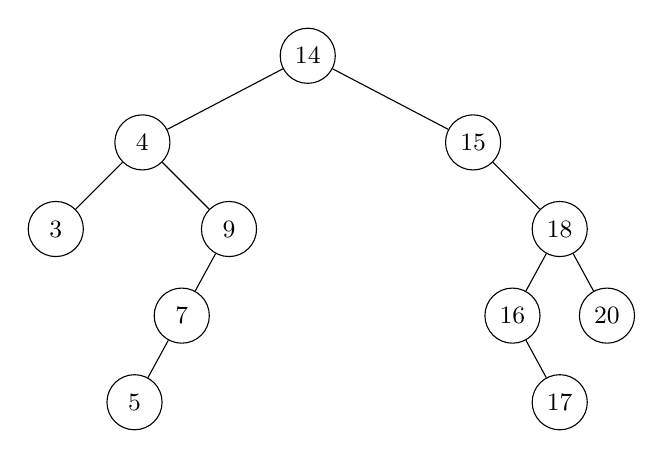
\begin{tikzpicture}[
    every node/.style={circle, draw, minimum size=7mm, inner sep=0pt, font=\small},
    level distance=11mm,
    level 1/.style={sibling distance=42mm},
    level 2/.style={sibling distance=22mm},
    level 3/.style={sibling distance=12mm}]
\node {14}
  child {node {4}
    child {node {3}}
    child {node {9}
      child {node {7}
        child {node {5}}
        child[missing]}
      child[missing]}}
  child {node {15}
    child[missing]
    child {node {18}
      child {node {16}
        child[missing]
        child {node {17}}}
      child {node {20}}}};
\end{tikzpicture}
\end{center}
檢查：這棵樹的前序是 14, 4, 3, 9, 7, 5, 15, 18, 16, 17, 20，和題目一樣。

\textbf{sortTree。} 二元搜尋樹的中序走訪（左子樹、根、右子樹）就是由小到大的順序（資結書
定理~9.1）：左子樹的鍵值都比根小、右子樹都比根大，遞迴下去每一段都排好了。 所以 sortTree 就是
遞迴的中序走訪：

\begin{code}{c}{由小到大印出二元搜尋樹}
struct node{
    int info;
    struct node *left;
    struct node *right;
};
typedef struct node *NODEPTR;

void sortTree(NODEPTR tree){
    if (tree == NULL)           /* 空樹：什麼都不印 */
        return;
    sortTree(tree->left);       /* 先印比根小的 */
    printf("%d ", tree->info);  /* 再印根 */
    sortTree(tree->right);      /* 最後印比根大的 */
}
\end{code}

對本題的樹輸出：3 4 5 7 9 14 15 16 17 18 20。

\textbf{複雜度。} 每個節點呼叫一次 \texttt{sortTree}、印一次，空指標的呼叫有 $n+1$ 個，時間
$\Theta(n)$；遞迴深度等於樹高 $h$，額外空間 $\Theta(h)$。 本題 $n = 11$，樹高 5（14--4--9--7--5
或 14--15--18--16--17）。
\end{pastsoln}
